%%%% paper.tex

\typeout{IJCAI--22 Instructions for Authors}

% These are the instructions for authors for IJCAI-22.

\documentclass{article}
\pdfpagewidth=8.5in
\pdfpageheight=11in
% The file ijcai22.sty is NOT the same as previous years'
\usepackage{ijcai22}

% Use the postscript times font!
\usepackage{times}
\usepackage{soul}
\usepackage{url}
\usepackage[hidelinks]{hyperref}
\usepackage[utf8]{inputenc}
\usepackage[small]{caption}
\usepackage{graphicx}
\usepackage{amsmath}
\usepackage{amsthm}
\usepackage{booktabs}
\usepackage{algorithm}
\usepackage{algorithmic}
\usepackage{makecell}
\usepackage{color}
\urlstyle{same}

% the following package is optional:
%\usepackage{latexsym}

% See https://www.overleaf.com/learn/latex/theorems_and_proofs
% for a nice explanation of how to define new theorems, but keep
% in mind that the amsthm package is already included in this
% template and that you must *not* alter the styling.
\newtheorem{example}{Example}
\newtheorem{theorem}{Theorem}

% Following comment is from ijcai97-submit.tex:
% The preparation of these files was supported by Schlumberger Palo Alto
% Research, AT\&T Bell Laboratories, and Morgan Kaufmann Publishers.
% Shirley Jowell, of Morgan Kaufmann Publishers, and Peter F.
% Patel-Schneider, of AT\&T Bell Laboratories collaborated on their
% preparation.

% These instructions can be modified and used in other conferences as long
% as credit to the authors and supporting agencies is retained, this notice
% is not changed, and further modification or reuse is not restricted.
% Neither Shirley Jowell nor Peter F. Patel-Schneider can be listed as
% contacts for providing assistance without their prior permission.

% To use for other conferences, change references to files and the
% conference appropriate and use other authors, contacts, publishers, and
% organizations.
% Also change the deadline and address for returning papers and the length and
% page charge instructions.
% Put where the files are available in the appropriate places.

% PDF Info Is REQUIRED.
% Please **do not** include Title and Author information
\pdfinfo{
/TemplateVersion (IJCAI.2022.0)
}

\title{Psychiatric Scale Guided Risky Post Screening for Early Depression Detection \\ (Appendix)}

\author{
Zhiling Zhang \and
Siyuan Chen \and
Mengyue Wu$^*$ \And
Kenny Zhu\thanks{Corresponding authors}
\affiliations
% $^1$First Affiliation\\
% $^2$Second Affiliation\\
% $^3$Third Affiliation\\
Shanghai Jiao Tong University
\emails
\{blmoistawinde, chensiyuan925, mengyuewu\}@sjtu.edu.cn,
kzhu@cs.sjtu.edu.cn
}

\begin{document}

\maketitle

\appendix

\section{Generalizability Tests}

Some studies have found that some existing depression detection models do not generalize well in the presence of distribution gaps among online-collected depression datasets \cite{harrigian2020models}. For instance, within 3 datasets collected from Reddit \cite{losada2016test,yates2017depression,wolohan2018detecting}, there are differences in the included subreddits, the time span of the posting histories, and the approaches to annotate the depressed users. As is suggested by \cite{ernala2019methodological}, current mental health prediction models tend to overfit on the characteristics of a specific dataset instead of learning what they claim to measure (i.e., a robust disease indicator). Therefore, even if there exists similarities for attempts in domain adaptation, the performance of current models still tend to degrade significantly. This highlights the difficulty for existing models to learn generalizable features. 

\subsection{Experimental Settings}

To test the generalizability of baseline models as well as the proposed method, we conduct experiments under conventional depression detection settings on 3 different datasets that have public availability and wide acceptance in previous works \cite{losada2017erisk,trotzek2018utilizing,harrigian2020models}. They are all collected from Reddit, but have different topic and label distribution and different content filtering strategy that aims to avoid label leakage and simulate user behaviors with different level of self-disclosure.\footnote{Although they label "depression" with different methods, they are all valid proxy signals of the same disease (``Depressive Disorder''), covering overlapping but slightly different subsets of patients. Therefore, the robustness across these depression subsets can indicate the general applicability of a method to some extent.} Besides eRisk2017, we introduce the two newly introduced datasets below. 

\paragraph{Topic-Restricted} consists of 6960 depressed users and 7683 control users, with a 8/1/1 random training/validation/test split \cite{wolohan2018detecting}. Since the original dataset is not released with the paper, we follow the implementation of \cite{harrigian2020models} to crawl the dataset ourselves in the same way. The depressed users are those who started a thread in depression subreddit while the control users are those who started a thread in AskReddit subreddit. The posting year spans from 2007 to 2021. For filtering, all posts in mental health related subreddits are removed. This stricter filtering strategy may further prevent model from overfitting on mental-health related signals, which can not be observed in depressed users who withhold their psychologic status due to the stigma of depression. 

\paragraph{RSDD} consists of 9210 depressed users and 107274 control users with a training/validation/test split of 39105/39122/39121, after data cleaning \cite{yates2017depression}. The depressed users are also identified with patterns, but further verified by annotators, while 12 control users are matched to a depressed user to minimize their distance of subreddit distribution. The posting year spans from 2006 to 2016. The filtering is the most strict among 3 datasets in that posts either posted in a mental health related subreddit or contain a depression-related term will be removed. This setting forces the model to learn the indirect signals for depression detection, so that they are more likely to detect the depression from patients with no self-report. However, it may also hinder the model's performance on those who would like to share their experience about depression.

For competing methods, we use the baselines described in \S 3, except HAN-GRU, BERT (Clus+Abs) for efficiency considerations. We additionally compare different variants of the proposed risky post screening strategy, including \textbf{Depress} using only 3 direct templates, \textbf{BDI-II} using 21 templates derived from BDI-II, and \textbf{Full} leveraging a combination of them (i.e. Psych described in \S 3). On the two new datasets, we find that a tiny version of BERT\footnote{https://huggingface.co/prajjwal1/bert-tiny} is enough to achieve competitive results given the larger data size. We select 64 posts, and train with batch size = 32 and learning rate = 2e-4. 

\subsection{In-domain Results}


\begin{table*}[t]
  \centering
\small
  \begin{tabular}{l|cccccc|c}
      \hline
          Source$\rightarrow$Target & T$\rightarrow$E & R$\rightarrow$E & E$\rightarrow$T & R$\rightarrow$T & E$\rightarrow$R & T$\rightarrow$R & Average  \\ 
          \hline
          LR & 82.6 & 72.3 & 68.8 & 67.3 & 77.8 & 52.0 & 70.1  \\
          Feature-rich & 85.7 & 75.3 & 69.6 & 73.3 & 77.6 & 52.7 & 72.4 \\ 
          \hline
          HAN-BERT (Depress) & 86.6 & 82.9 & 75.8 & 71.1 & 82.6 & \textbf{74.8} & 79.0  \\
          HAN-BERT (BDI-II) & \textbf{87.6} & 83.8 & 74.9 & \textbf{74.6} & 80.4 & 73.5 & 79.1  \\
          HAN-BERT (Full) & 87.4 & \textbf{85.0} & \textbf{77.5} & 72.4 & \textbf{84.4} & 72.3 & \textbf{79.8} \\ 
          \hline
      \end{tabular}
  \caption{Cross-domain experimental results (AUC) between eRisk2017(E), Topic-Restricted(T) and RSDD(R).}
  \label{table:cross} 
\end{table*}

\begin{table}[t]
  \centering
  \small
  \begin{tabular}{l|cc}
      \hline
      {} & Topic-Restricted & RSDD \\
      \hline
      LR & 69.8 & 52.1 \\
      Feature-Rich & 72.0 & 58 \\
      \hline
      BERT (Clus) & 56.7 & - \\
      HAN-BERT$_{tiny}$ (Heuristic) & 68.0 & 38.2 \\
      HAN-BERT$_{tiny}$ (Clus) & 71.9 & - \\
      \hline
      HAN-BERT$_{tiny}$ (Depress) & 77.1 & \textbf{65.4} \\
      HAN-BERT$_{tiny}$ (BDI-II) & \textbf{78.9} & 60.1 \\
      HAN-BERT$_{tiny}$ (Full) & 77.1 & 61.1 \\
      \hline
  \end{tabular}
  \caption{Test F1 on Topic-Restricted and RSDD dataset.}
  \label{table:rsdd_wolohan} 
\end{table}

The in-domain results on the 2 new datasets are shown in Table \ref{table:rsdd_wolohan}. BERT (Clus) and HAN-BERT (Clus) don't show competitive performance on Topic-Restricted again while requiring expensive clustering stage, so we don't experiment them on the larger RSDD dataset. The proposed risky post screening based methods show strong performance, and are capable of outperforming both the traditional Feature-Rich (all posts) using only 64 posts and a tiny version of BERT. The orders between these screening methods differ across datasets possibly due to their differences in label distribution and filtering strategy, but their performances are overall competitive.

\subsection{Cross-domain Results}

To test the cross-domain generalizability of different approaches, we train models on a source dataset and directly test the model on another target dataset for all 6 possible combinations of the 3 datasets. For HAN-BERT models, we use the model trained with 16 selected posts, and also test on 16 posts selected with the same templates. In contrast to in-domain experiments using a fixed probability threshold 0.5 to decide the prediction, we don't apply this in cross-domain tests since the label distribution differs greatly between datasets, so that fixed threshold will lead to poor performance. Instead, we use a threshold-free metric, AUC, to measure the performance of each method.

The results are shown in Table \ref{table:cross}. Consistent with in-domain results, we find that Feature-Rich outperforms LR in terms of average domain adaptation AUC. Moreover, the performance of all HAN-BERT models are more robust than baselines, which suggests the generalizability of the proposed method.

We then analyze the results in detail. The performance of LR and Feature-rich degrade significantly in the T$\rightarrow$R setting. We hypothesize that the reason lies in the different annotation strategy for depressed and control users. Topic-Restricted treats users who started a thread in depression/AskReddit subreddit as depressed/control users and does not control the similarities between the 2 groups, while RSDD specifically selects control users with similar subreddit distribution as depressed users. Therefore, the baselines may have learned spurious clues about the annotation strategy of Topic-Restricted. For example, we checked the coefficients of the LR model, and found that words like ``askreddit'' and ``redditors'' are among the most important features for the decision of control users. In contrast, HAN-BERT models still exhibit satisfying performance, which suggests that they can leverage robust depression indicators. 

LR and Feature-Rich perform much worse than HAN-BERT models in both direction between RSDD and eRisk2017. These two datasets adopts different filtering strategies, where eRisk2017 preserves most posts while RSDD excludes all posts in mental health related subreddits or containing a depression-related term. The results indicate that HAN-BERT models are less affected by such domain gap. 

HAN-BERT models also significantly outperform baselines in the E$\rightarrow$T and E$\rightarrow$R settings, which shows that they can effectively capture depression signals even with the extremely small eRisk2017 dataset. Comparing all variants of HAN-BERT models, HAN-BERT (Full) shows the best average performance, which indicates the usefulness of combining the theory-guided templates with direct depression indicators in selecting robust features across domains. Therefore, HAN-BERT (Full) can be a preferred choice in real world applications where the target domain distribution is unknown, and we select this variant as the representative of the proposed method.

\section{Lexical Analysis}

\begin{figure*}[t]
    \centering
    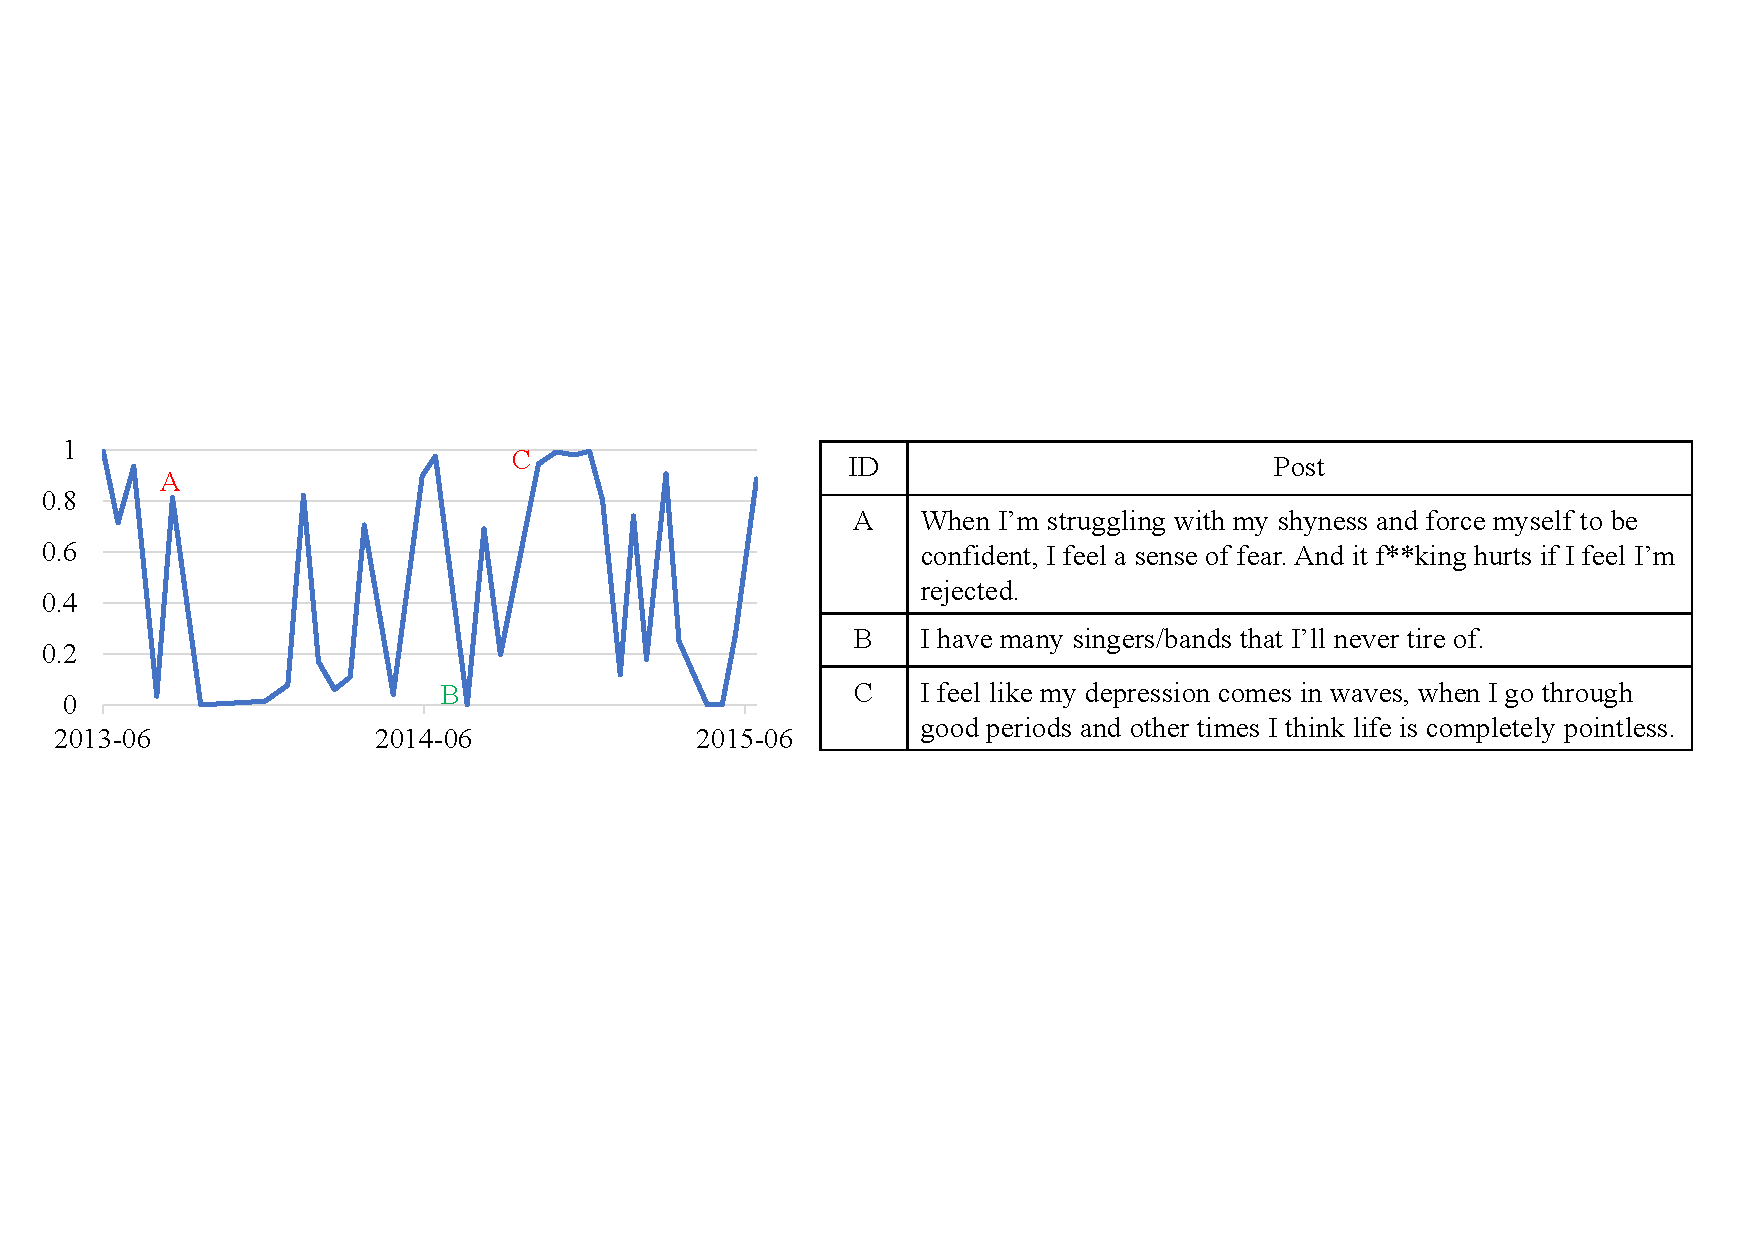
\includegraphics[width=2\columnwidth]{figures/curve.pdf}
    \caption{Predicted depression score by HAN-BERT (Full) along with time for a user in eRisk2017 dataset. We selected 3 time periods on predicted peaks and troughs, and show a representative post in each period.}
    \label{fig:curve}
\end{figure*}

As has been shown in many previous works \cite{shen2017depression,eichstaedt2018facebook,wolohan2018detecting}, there are many significant lexical differences between the posts of depressed users and other users, which can be captured by the word frequency of certain categories in LIWC \cite{pennebaker2001linguistic}. For example, depressed users tend to use more \textbf{first person pronouns} (\textit{I}), words expressing \textbf{negative emotions} (e.g. \textit{hate, miss, alone}), and words about \textbf{health} (e.g. \textit{life, tired, sick}). Such lexical discrepancies do not only exist between the two groups of users, but also within the posts of depressed users themselves. Therefore, we run risky post screening on the posts of depressed users in the eRisk2017 test set, and count the frequency of words in the 3 LIWC categories stated above. We then compare the proportion of these words in selected posts and other posts, and test their differences with two-sided proportion $z$ test. If the selected posts show stronger lexical depression indicators, we can further confirm the helpfulness of risky post screening in capturing reliable depression features.

\begin{figure}[h]
  \centering
  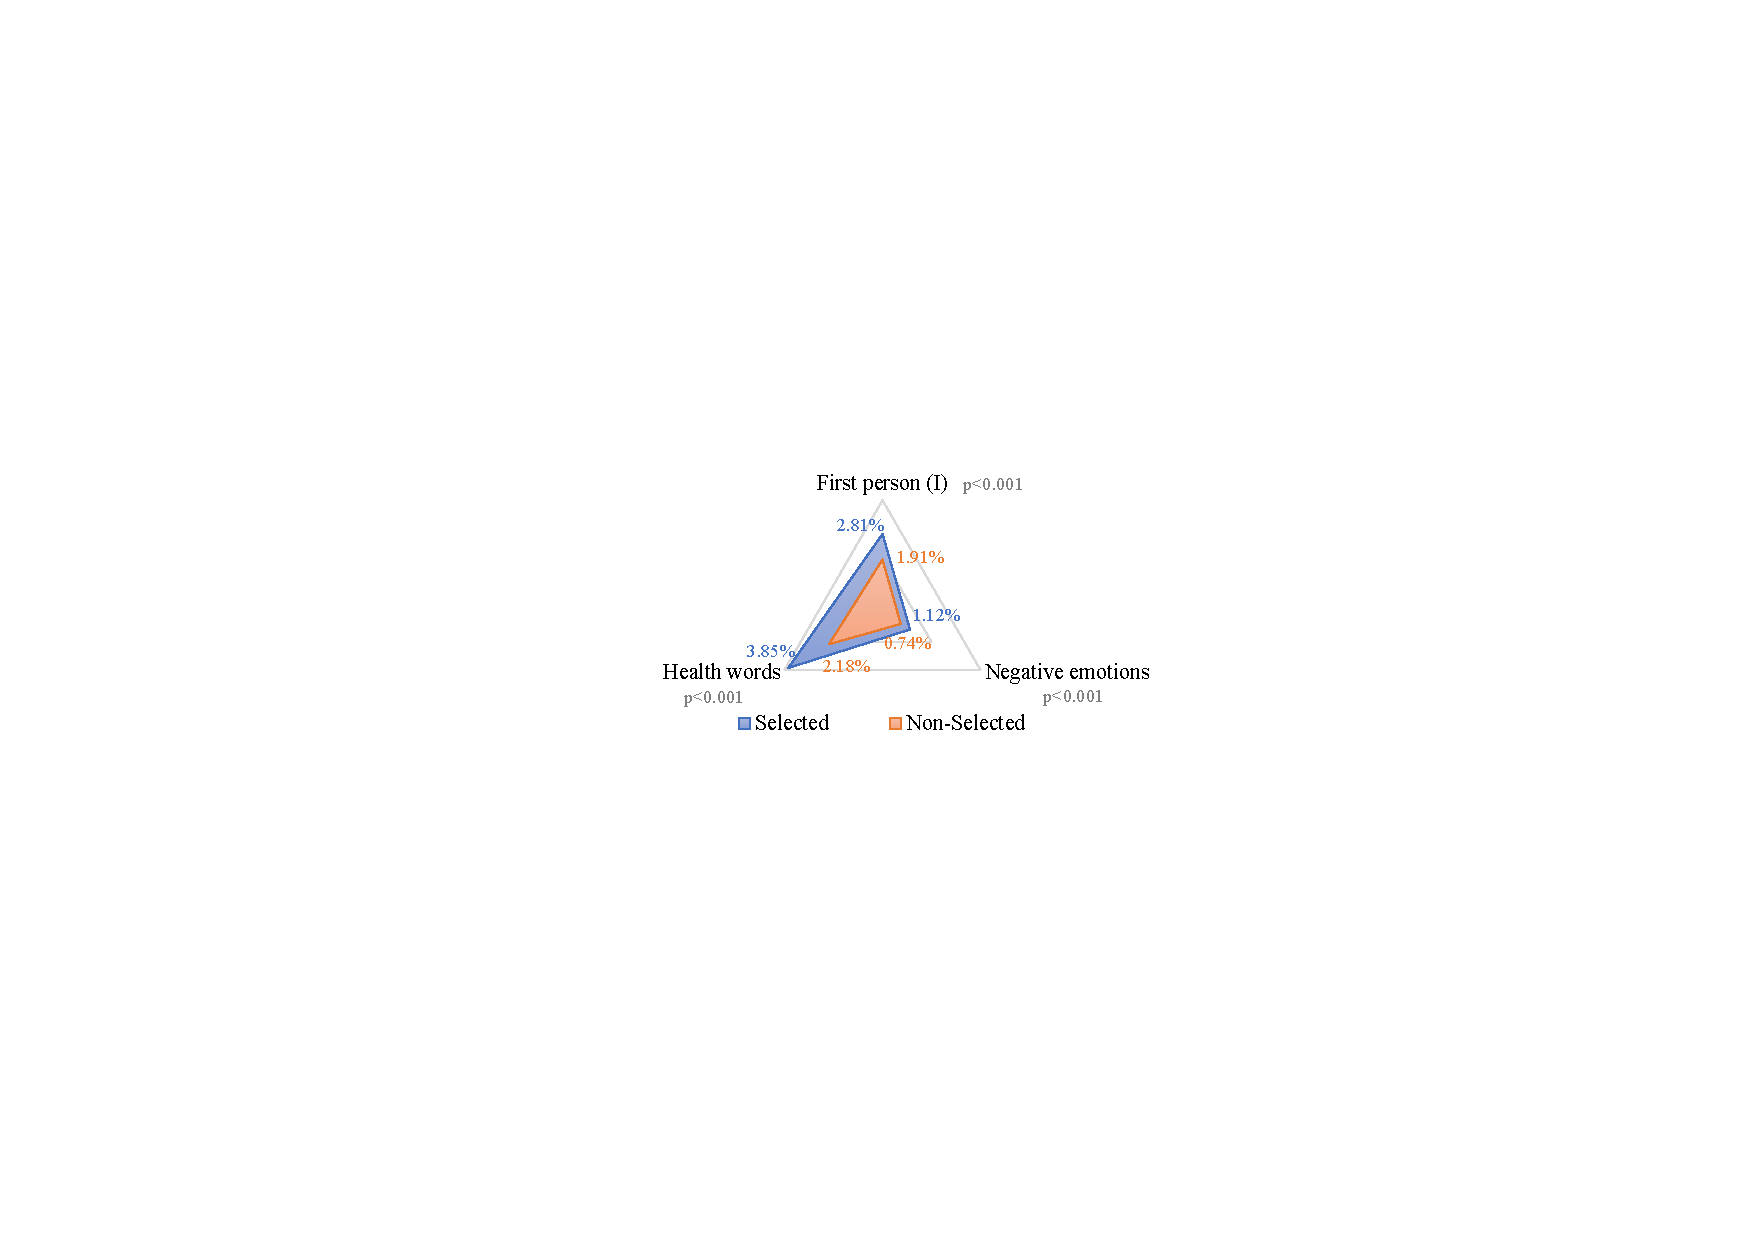
\includegraphics[width=0.88\columnwidth]{figures/lexical.pdf}
  \caption{Difference between selected and non-selected posts w.r.t. proportion of words in typical depress related LIWC categories.}
  \label{fig:lexical}
\end{figure}

As is illustrated in Figure \ref{fig:lexical}, there are significant differences between the use of first person words, negative emotions and health-related words in selected (risky) and non-selected posts ($p < 0.001$ for all categories). The difference between risky posts and other posts of depressed users (Negative Emotion: 1.12\% vs. 0.74\%) can be even bigger than the difference between non-risky posts of depressed users and all posts from non-depressed users (Negative Emotion: 0.74\% vs. 0.79\%). These findings are similar to those reported in previous literature, which verifies the convergent validity of the proposed method.

\section{Temporal Analysis}

We also demonstrate that our method has the potential to track the fluctuations in depressive mood for depression patients by another example (Figure \ref{fig:curve}). We produce such curve with the following procedure. First, we group posts according to a 14-day interval. Then we use HAN-BERT (Full) to conduct post screening and depression detection to get a predicted probability for each post group. To produce a smooth curve along time, we design a moving average strategy to derive a more stable depression score from predicted depression probabilities. Suppose the predicted probability of group $i$ is $pr_i$, and the depression score is $s_i$. Then we have 
$$s_1 = pr_1, s_i = \alpha s_{i-1} + (1-\alpha) pr_{i-1} (i > 1)$$
where $\alpha = max(0, 0.5 * \frac{28-t_{\Delta}}{28-1})$, $t_{\Delta}$ is the time interval between the first post of two groups measured in days. Therefore, if two groups are close in time, then the score from the last period will have a higher influence on the next score. Finally, we plot the curve according to the moving-averaged scores.


As we can see in Figure \ref{fig:curve}. In addition to the accurate detection of depression, the proposed method may also be able to capture the changes in the severity of depression symptoms. The model reported a high risk when the user expressed typical depression symptoms like frustrations (A) or worthlessness (C), and also reported low depression score when the user actually showed interest in things (B), which might indicate a recovery from the symptom of ``Loss of Interest''. The overall trend is in line with the user's self-report that the depression comes cyclically like waves.

\section{Hyperparameter Analysis}
\label{sec:factor}

Here we study the impact of 2 hyperparameters of risky post screening.

\paragraph{Number of Posts} 
We study the effect of post numbers on the Topic-Restricted dataset (Figure \ref{fig:post_numbers}). It can be seen that all methods can get further improvement given more posts, and scale-based methods can benefit more possibly because more posts can help cover more diverse expressions of depression symptoms, which cannot be fully captured given a small size limit.

\begin{figure}[h]
    \centering
    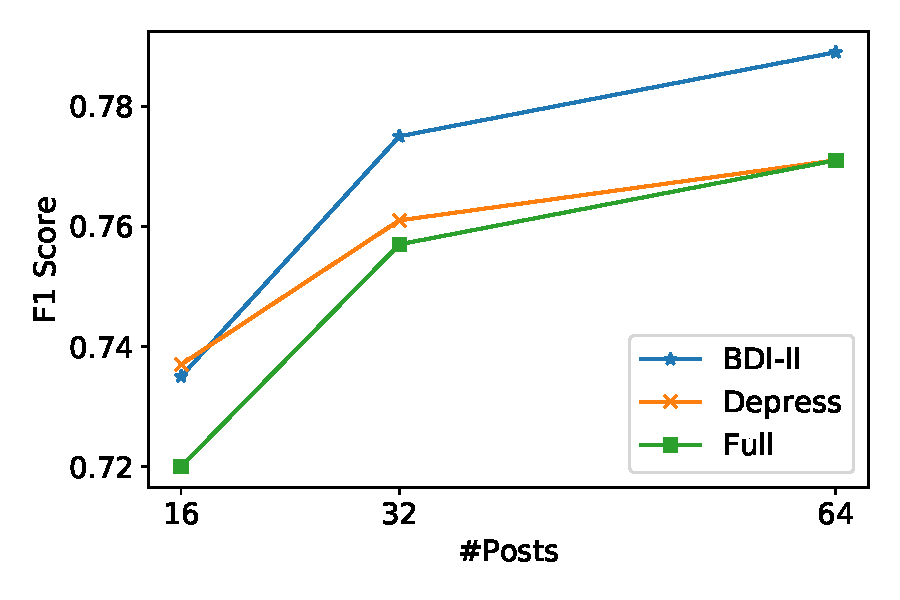
\includegraphics[width=0.8\columnwidth]{figures/post_numbers.pdf}
    \caption{Effect of number of posts on Topic-Restricted.}
    \label{fig:post_numbers}
\end{figure}

\paragraph{Different Scales}
We explore three other commonly-adopted scales besides BDI-II, including HDRS \cite{hamilton1986hamilton}, CES-D \cite{Lenore1977CES-D} and PHQ-9 \cite{kroenke2001phq}, with similar approaches to rewrite the dimensions into depression templates. We also tried Majority Voting of models paired with different scales. Their performance on eRisk2017 dataset in shown in Table \ref{tab:scales}. We found that BDI-II is the single best performing scale. The combination of HDRS, BDI-II and PHQ-9 reaches the highest performance for their highly complementary dimensions. 

\begin{table}[h]
    \centering
	\small
    \begin{tabular}{l|c}
        \hline
        Depression Scale & F1 \\
        \hline
        BDI-II & \textbf{70.3} \\
        HDRS & 68.0 \\
        CES-D & 67.9 \\
        PHQ-9 & 67.2\\
        \hline
        HDRS+BDI-II+PHQ-9 & \textbf{72.1} \\
        HDRS+BDI-II+CES-D & 70.5 \\
        \hline
    \end{tabular}
    \caption{Test results on eRisk2017 dataset with different depression scales and their combinations.}
    \label{tab:scales}
\end{table}

\section{Depression Templates}

Here we provide the templates in detail. We mainly use a combination of 3 direct depression descriptions and the 21 indirect symptoms derived from BDI-II (Table \ref{tab:BDI-II}) \cite{beck1996beck}. As is mentioned in \S \ref{sec:factor}, we also experimented other well-known depression scales like HDRS (Table \ref{tab:Hamilton}) \cite{hamilton1986hamilton}, CES-D (Table \ref{tab:CES-D}) \cite{Lenore1977CES-D} and PHQ-9 (Table \ref{tab:PHQ-9}) \cite{kroenke2001phq}. The original scales usually contain different descriptions under the same dimension to distinguish different level of intensity or frequency. However, we find that current sentence representations have difficulty in capturing such nuanced differences. We thus condense the descriptions of each dimension into one general template (A few may have more, if there are significant intra-dimension difference).

\begin{table}
  \centering
  \small
  \begin{tabular}{l|l}
  \hline
  Dimension & Template \\
  \hline
  Feeling Depressed  &  I feel depressed. \\
  Diagnosis &  I am diagnosed with depression. \\
  Treatment &  I am treating my depression. \\
  \hline
  Sadness & I feel sad.  \\
  Pessimism & I am discouraged about my future.  \\
  Past Failure & I always fail. \\
  Loss of Pleasure & I don't get pleasure from things. \\
  Guilty Feelings & I feel quite guilty. \\
  Punishment Feelings & I expected to be punished. \\
  Self-Dislike & I am disappointed in myself. \\
  Self-Criticalness & I always criticize myself for my faults. \\
  Suicidal Thoughts or Wishes & I have thoughts of killing myself. \\
  Crying & I always cry. \\
  Agitation & I am hard to stay still. \\
  Loss of Interest & It's hard to get interested in things. \\
  Indecisiveness & I have trouble making decisions. \\
  Worthlessness & I feel worthless. \\
  Loss of Energy & I don't have energy to do things. \\
  Changes in Sleeping Pattern & I have changes in my sleeping pattern. \\
  Irritability & I am always irritable. \\
  Changes in Appetite & I have changes in my appetite. \\
  Concentration Difficulty & I feel hard to concentrate on things. \\
  Tiredness  & I am too tired to do things. \\
  Loss of Interest in Sex & I have lost my interest in sex. \\
  \hline
  \end{tabular}
  \caption{The main templates and their corresponding dimensions we used in our experiments, including 3 direct depression descriptions and 21 indirect symptoms derived from BDI-II. }
  \label{tab:BDI-II} 
\end{table}


\begin{table}
    \centering
    \small
    \begin{tabular}{l}
      \hline
      I have depressed mood. \\
      I always feel sad. \\
      I feel hopeless. \\
      I feel helpless. \\
      I find myself worthless. \\
      I have feelings of guilty. \\
      I always let people down. \\
      I feel like I should be punished. \\
      I think life is not worth living. \\
      I have thoughts of killing myself. \\
      I tried to suicide. \\
      I have difficulty falling asleep. \\
      I feel restless. \\
      I always wake up during the night. \\
      I have lost my interest in many things. \\
      I decrease time spent in my job. \\
      I find it difficult to concentrate on things. \\
      I can not stay still. \\
      I always worry about small things. \\
      I am irritable. \\
      I feel anxiety. \\
      I have a bad appetite. \\
      I am easy to be tired. \\
      I have less interest in sex. \\
      I suffers from menstrual disturbances. \\
      I worry about my health. \\
      I lose weight dramatically. \\
      \hline
    \end{tabular}
    \caption{The templates adapted from the HDRS depression scale. }
    \label{tab:Hamilton} 
  \end{table}
  
  \begin{table}
    \centering
    \small
    \begin{tabular}{l}
      \hline
      I am bothered by things that usually don't bother me. \\
      I do not feel like eating. \\
      My appetite is poor. \\
      I feel that I could not shake off the blues even with help \\
      -from my family or friends. \\
      I am not just as good as other people. \\
      I have trouble keeping my mind on what I am doing. \\
      I feel depressed. \\
      I feel that everything I did was an effort. \\
      I feel hopeless about the future. \\
      I thought my life had been a failure. \\
      I feel fearful. \\
      My sleep is restless. \\
      I am unhappy. \\
      I talk less than usual. \\
      I feel lonely. \\
      I think people are unfriendly. \\
      It's difficult for me to enjoy life. \\
      I had crying spells. \\
      I feel sad. \\
      I feel that people dislike me. \\
      I could not get 'going'. \\
      \hline
    \end{tabular}
    \caption{The templates adapted from the CES-D depression scale. }
    \label{tab:CES-D} 
  \end{table}
  
  \begin{table}
    \centering
    \small
    \begin{tabular}{l}
      \hline
      I have little interest in doing things. \\
      I have little pleasure in doing things. \\
      I always feel down. \\
      I always depressed. \\
      I always hopeless. \\
      I have trouble falling asleep. \\
      I sleep too much. \\
      I feel tired. \\
      I have little energy. \\
      My appetite is poor. \\
      I cannot stop overeating. \\
      I feel bad about myself. \\
      I think myself a failure. \\
      I have let other people down. \\
      I have trouble concentrating on things. \\
      I move much slower than before. \\
      I speak much slower than before. \\
      I have been moving around a lot more than usual. \\
      I think that I would be better off dead. \\
      I have thoughts of hurting myself. \\
      \hline
    \end{tabular}
    \caption{The templates adapted from the PHQ-9 depression scale. }
    \label{tab:PHQ-9} 
  \end{table}

\section{Ethical and Broader Impact Statement}

This work aims to help people suffering from depression, but have not yet been diagnosed due to the difficulty in receiving clinical help or the stigmatization of the disease. It can be a sensitive topic so it is important to discuss the potential risks and limitations of our work. The proposed method can conduct early depression detection on social media. However, the performance is far from prefect, so the models' early alerts still require careful examinations from professional practitioners. The proposed method can provide diagnostic bases as explanations, but the diagnostic basis may not precisely matched the actual symptom implied in the post. Therefore, the diagnostic basis should be checked before adoption. Moreover, the datasets are annotated with proxy signals of depression, which may not be representative of the true population of depression patients. In practice, the model should be trained on a more carefully-curated dataset for reliable predictions.

The datasets used in this work are either publicly available or used under their corresponding data usage agreement. All posts in examples were de-identified and paraphrased for anonymity.

%% The file named.bst is a bibliography style file for BibTeX 0.99c
\bibliographystyle{named}
\bibliography{paper}

\end{document}


